% Options for packages loaded elsewhere
% Options for packages loaded elsewhere
\PassOptionsToPackage{unicode}{hyperref}
\PassOptionsToPackage{hyphens}{url}
\PassOptionsToPackage{dvipsnames,svgnames,x11names}{xcolor}
%
\documentclass[
  12pt,
]{article}
\usepackage{xcolor}
\usepackage[paperwidth=42in,paperheight=25in,top=.2in,bottom=0.5in,left=0.5in,right=0.5in,columnsep=0.75in]{geometry}
\usepackage{amsmath,amssymb}
\setcounter{secnumdepth}{-\maxdimen} % remove section numbering
\usepackage{iftex}
\ifPDFTeX
  \usepackage[T1]{fontenc}
  \usepackage[utf8]{inputenc}
  \usepackage{textcomp} % provide euro and other symbols
\else % if luatex or xetex
  \usepackage{unicode-math} % this also loads fontspec
  \defaultfontfeatures{Scale=MatchLowercase}
  \defaultfontfeatures[\rmfamily]{Ligatures=TeX,Scale=1}
\fi
\usepackage{lmodern}
\ifPDFTeX\else
  % xetex/luatex font selection
\fi
% Use upquote if available, for straight quotes in verbatim environments
\IfFileExists{upquote.sty}{\usepackage{upquote}}{}
\IfFileExists{microtype.sty}{% use microtype if available
  \usepackage[]{microtype}
  \UseMicrotypeSet[protrusion]{basicmath} % disable protrusion for tt fonts
}{}
\usepackage{setspace}
\makeatletter
\@ifundefined{KOMAClassName}{% if non-KOMA class
  \IfFileExists{parskip.sty}{%
    \usepackage{parskip}
  }{% else
    \setlength{\parindent}{0pt}
    \setlength{\parskip}{6pt plus 2pt minus 1pt}}
}{% if KOMA class
  \KOMAoptions{parskip=half}}
\makeatother
% Make \paragraph and \subparagraph free-standing
\makeatletter
\ifx\paragraph\undefined\else
  \let\oldparagraph\paragraph
  \renewcommand{\paragraph}{
    \@ifstar
      \xxxParagraphStar
      \xxxParagraphNoStar
  }
  \newcommand{\xxxParagraphStar}[1]{\oldparagraph*{#1}\mbox{}}
  \newcommand{\xxxParagraphNoStar}[1]{\oldparagraph{#1}\mbox{}}
\fi
\ifx\subparagraph\undefined\else
  \let\oldsubparagraph\subparagraph
  \renewcommand{\subparagraph}{
    \@ifstar
      \xxxSubParagraphStar
      \xxxSubParagraphNoStar
  }
  \newcommand{\xxxSubParagraphStar}[1]{\oldsubparagraph*{#1}\mbox{}}
  \newcommand{\xxxSubParagraphNoStar}[1]{\oldsubparagraph{#1}\mbox{}}
\fi
\makeatother


\usepackage{longtable,booktabs,array}
\usepackage{calc} % for calculating minipage widths
% Correct order of tables after \paragraph or \subparagraph
\usepackage{etoolbox}
\makeatletter
\patchcmd\longtable{\par}{\if@noskipsec\mbox{}\fi\par}{}{}
\makeatother
% Allow footnotes in longtable head/foot
\IfFileExists{footnotehyper.sty}{\usepackage{footnotehyper}}{\usepackage{footnote}}
\makesavenoteenv{longtable}
\usepackage{graphicx}
\makeatletter
\newsavebox\pandoc@box
\newcommand*\pandocbounded[1]{% scales image to fit in text height/width
  \sbox\pandoc@box{#1}%
  \Gscale@div\@tempa{\textheight}{\dimexpr\ht\pandoc@box+\dp\pandoc@box\relax}%
  \Gscale@div\@tempb{\linewidth}{\wd\pandoc@box}%
  \ifdim\@tempb\p@<\@tempa\p@\let\@tempa\@tempb\fi% select the smaller of both
  \ifdim\@tempa\p@<\p@\scalebox{\@tempa}{\usebox\pandoc@box}%
  \else\usebox{\pandoc@box}%
  \fi%
}
% Set default figure placement to htbp
\def\fps@figure{htbp}
\makeatother


% definitions for citeproc citations
\NewDocumentCommand\citeproctext{}{}
\NewDocumentCommand\citeproc{mm}{%
  \begingroup\def\citeproctext{#2}\cite{#1}\endgroup}
\makeatletter
 % allow citations to break across lines
 \let\@cite@ofmt\@firstofone
 % avoid brackets around text for \cite:
 \def\@biblabel#1{}
 \def\@cite#1#2{{#1\if@tempswa , #2\fi}}
\makeatother
\newlength{\cslhangindent}
\setlength{\cslhangindent}{1.5em}
\newlength{\csllabelwidth}
\setlength{\csllabelwidth}{3em}
\newenvironment{CSLReferences}[2] % #1 hanging-indent, #2 entry-spacing
 {\begin{list}{}{%
  \setlength{\itemindent}{0pt}
  \setlength{\leftmargin}{0pt}
  \setlength{\parsep}{0pt}
  % turn on hanging indent if param 1 is 1
  \ifodd #1
   \setlength{\leftmargin}{\cslhangindent}
   \setlength{\itemindent}{-1\cslhangindent}
  \fi
  % set entry spacing
  \setlength{\itemsep}{#2\baselineskip}}}
 {\end{list}}
\usepackage{calc}
\newcommand{\CSLBlock}[1]{\hfill\break\parbox[t]{\linewidth}{\strut\ignorespaces#1\strut}}
\newcommand{\CSLLeftMargin}[1]{\parbox[t]{\csllabelwidth}{\strut#1\strut}}
\newcommand{\CSLRightInline}[1]{\parbox[t]{\linewidth - \csllabelwidth}{\strut#1\strut}}
\newcommand{\CSLIndent}[1]{\hspace{\cslhangindent}#1}



\setlength{\emergencystretch}{3em} % prevent overfull lines

\providecommand{\tightlist}{%
  \setlength{\itemsep}{0pt}\setlength{\parskip}{0pt}}



 


\usepackage[T1]{fontenc}       % Use modern font encoding
\usepackage{helvet}            % Use Helvetica clone (sans-serif)
\renewcommand\familydefault{\sfdefault} % Make sans-serif the default font family
\usepackage{graphicx}          % Required for images
\usepackage{amsmath}           % For math symbols if needed
\usepackage{amssymb}           % For math symbols if needed
\usepackage{textcomp}          % For symbols like degrees
\usepackage{xcolor}            % For color definitions
\usepackage{multicol}          % For multi-column layout
\usepackage{geometry}          % To set paper size and margins (already used by Quarto, but good practice)
\usepackage{fancyhdr}          % For headers and footers
% \usepackage{titlesec}          % For customizing section titles
\usepackage{sectsty}           % Alternative/complement to titlesec for section fonts
\usepackage{enumitem}          % For customizing lists (itemize, enumerate)
\usepackage{caption}           % For customizing figure/table captions
\usepackage{subcaption} 
\usepackage{hyperref}          % For clickable links (references, URLs)
\usepackage{tikz}              % For drawing header/footer backgrounds
\usepackage{subcaption}
\usepackage{amsfonts}
\usepackage{etoolbox}
\usepackage{titletoc}        % For table of contents customization
\usepackage[explicit]{titlesec}  % For section title customization with explicit option
\usepackage{caption}
\captionsetup[figure]{labelformat=empty}% redefines the caption setup of the figures environment in the beamer class.


% --- Color Definitions ---
\definecolor{purduegold}{HTML}{CEB888} % Keep original Purdue Gold
\definecolor{purdueblack}{HTML}{000000}
\definecolor{purduegray}{HTML}{5F6062}  % Keep original Purdue Gray
\definecolor{sectionbg}{HTML}{D6C8A3}  % New tan/beige color for section headers
\definecolor{lightgold}{HTML}{FBF8F1}  % A lighter shade for backgrounds
\definecolor{darkgray}{HTML}{333333}   % Darker Gray for text contrast

% --- SET BASE FONT SIZE HERE (Overrides any default/cached \normalsize) ---
\makeatletter
\renewcommand{\normalsize}{%
    \@setfontsize\normalsize{19.5pt}{22pt}% Main font size and line spacing
    \abovedisplayskip 12pt plus 3pt minus 7pt
    \abovedisplayshortskip \z@ plus 3pt
    \belowdisplayshortskip 6.5pt plus 3.5pt minus 3pt
    \belowdisplayskip \abovedisplayskip
    \let\@listi\@listI}
\makeatother

% Adjust other font size commands to be in proportion to normalsize
\makeatletter
\renewcommand{\large}{\@setfontsize\large{18pt}{24pt}}
\renewcommand{\Large}{\@setfontsize\Large{20pt}{26pt}}
\renewcommand{\LARGE}{\@setfontsize\LARGE{24pt}{30pt}}
\renewcommand{\huge}{\@setfontsize\huge{28pt}{36pt}}
\renewcommand{\Huge}{\@setfontsize\Huge{34pt}{42pt}}
\makeatother

\normalsize  % Activate the new normal size definition


% --- Font & Section Styling ---
% Using sectsty for simplicity here
\sectionfont{\color{darkgray}\huge\bfseries\sffamily\raggedright} % Make section titles large, bold, dark gray
\subsectionfont{\color{darkgray}\Large\bfseries\sffamily\raggedright} % Make subsection titles large, bold, dark gray
\subsubsectionfont{\color{purduegray}\large\bfseries\sffamily\raggedright} % Make subsubsection titles medium, bold, gray

% --- ADJUST SPACING HERE ---
% Reduce space AFTER section titles and BEFORE subsections/subsubsections
% Format: \titlespacing*{<command>}{<left>}{<before-sep>}{<after-sep>}
\titlespacing*{\section}
  {0pt}               % Left margin
  {.3ex plus 0.2ex minus .0ex} % Space BEFORE title (reduced slightly)
  {0.3ex plus .1ex}   % Space AFTER title (SIGNIFICANTLY REDUCED from 1ex or more)

\titlespacing*{\subsection}
  {0pt}               % Left margin
  {.1ex plus 0.1ex minus .0ex} % Space BEFORE title (reduced slightly)
  {0.1ex plus .1ex}   % Space AFTER title (REDUCED)

\titlespacing*{\subsubsection}
  {0pt}               % Left margin
  {0.1ex plus 0.1ex minus .2ex} % Space BEFORE title (reduced slightly)
  {0.0ex plus .02ex}   % Space AFTER title (REDUCED)

% --- List Styling ---
\setlist[itemize]{leftmargin=1.5em, label=\textbullet, itemsep=0.4ex, topsep=0.05ex} % Adjust bullet indentation and spacing
\setlist[enumerate]{leftmargin=1.5em, itemsep=0.2ex, topsep=0.5ex}

% --- ADJUST LIST SPACING HERE ---
% Reduce space BEFORE the entire list starts
\setlist[itemize]{
  leftmargin=1.5em,     % Indentation
  label=\textbullet,    % Bullet style
  itemsep=0.2ex,        % Space between items in the list
  topsep=0.0ex          % Space BEFORE the first item (SIGNIFICANTLY REDUCED from 0.5ex or more)
}
\setlist[enumerate]{
  leftmargin=1.5em,
  itemsep=0.2ex,
  topsep=0.2ex          % Space BEFORE the first item (REDUCED)
}


% --- Section Header Styling ---
% Define the section background color first
\definecolor{sectionbg}{HTML}{D6C8A3}  % Tan/beige color for section headers

% Use a simpler approach for section styling without relying on TikZ nodes
\titleformat{\section}
  {\normalfont\Large\bfseries\sffamily}
  {}
  {0pt}
  {\colorbox{sectionbg}{\parbox{\dimexpr\columnwidth-2\fboxsep\relax}{\centering#1}}}
  []

% For unnumbered sections
\titleformat{name=\section,numberless}
  {\normalfont\Large\bfseries\sffamily}
  {}
  {0pt}
  {\colorbox{sectionbg}{\parbox{\dimexpr\columnwidth-2\fboxsep\relax}{\centering#1}}}
  []

% Adjust spacing around sections
\titlespacing*{\section}
  {0pt}
  {1.5ex plus 0.5ex minus 0.2ex}
  {1.0ex plus 0.2ex}

% --- Header and Footer Styling ---
\pagestyle{fancy} % Use fancyhdr
\fancyhf{}       % Clear default header/footer
\renewcommand{\headrulewidth}{0pt} % No header rule
\renewcommand{\footrulewidth}{0pt} % No footer rule
% Footer content is added via tikz overlay in after-body.tex


\DeclareCaptionFont{subcapstyle}{\sffamily\fontsize{16pt}{19pt}\selectfont}

% --- Figure Caption Styling ---
\captionsetup{
  font={normalsize, sf},          % Small sans-serif font for captions
  labelfont={bf, color=darkgray}, % Bold, dark gray label (e.g., "Figure 1:")
  labelsep=period,           % Use period after label
  justification=raggedright, % Left-align caption text
  singlelinecheck=false,     % Ensure justification applies even to single lines
  skip=1ex                   % Space between figure and caption
}

\captionsetup[subfigure]{font=subcapstyle} 


% --- Hyperlink Styling ---
\hypersetup{
  colorlinks=true,          % Enable colored links
  linkcolor=purduegray,     % Color for internal links (e.g., refs)
  citecolor=purduegray,     % Color for citation links
  filecolor=purduegray,     % Color for file links
  urlcolor=purduegray,      % Color for URL links
  pdftitle={Planning to Save Energy: How Information Format Affects Accuracy}, % PDF metadata
  pdfauthor={Thomas E. Gorman et al.} % PDF metadata
}
\AtBeginEnvironment{CSLReferences}{\footnotesize} 
\makeatletter
\@ifpackageloaded{caption}{}{\usepackage{caption}}
\AtBeginDocument{%
\ifdefined\contentsname
  \renewcommand*\contentsname{Table of contents}
\else
  \newcommand\contentsname{Table of contents}
\fi
\ifdefined\listfigurename
  \renewcommand*\listfigurename{List of Figures}
\else
  \newcommand\listfigurename{List of Figures}
\fi
\ifdefined\listtablename
  \renewcommand*\listtablename{List of Tables}
\else
  \newcommand\listtablename{List of Tables}
\fi
\ifdefined\figurename
  \renewcommand*\figurename{Figure}
\else
  \newcommand\figurename{Figure}
\fi
\ifdefined\tablename
  \renewcommand*\tablename{Table}
\else
  \newcommand\tablename{Table}
\fi
}
\@ifpackageloaded{float}{}{\usepackage{float}}
\floatstyle{ruled}
\@ifundefined{c@chapter}{\newfloat{codelisting}{h}{lop}}{\newfloat{codelisting}{h}{lop}[chapter]}
\floatname{codelisting}{Listing}
\newcommand*\listoflistings{\listof{codelisting}{List of Listings}}
\makeatother
\makeatletter
\makeatother
\makeatletter
\@ifpackageloaded{caption}{}{\usepackage{caption}}
\@ifpackageloaded{subcaption}{}{\usepackage{subcaption}}
\makeatother
\usepackage{bookmark}
\IfFileExists{xurl.sty}{\usepackage{xurl}}{} % add URL line breaks if available
\urlstyle{same}
\hypersetup{
  pdftitle={Planning to Save Energy: How Information Format Affects Accuracy},
  colorlinks=true,
  linkcolor={blue},
  filecolor={Maroon},
  citecolor={Blue},
  urlcolor={Blue},
  pdfcreator={LaTeX via pandoc}}


\title{Planning to Save Energy: How Information Format Affects Accuracy}
\author{}
\date{}
\begin{document}
% before-body.tex

% Replace the current header background with a more subtle approach
\AddToHook{shipout/background}{% Add to background hook for each page
  \begin{tikzpicture}[remember picture, overlay]
    % Fill header area with a much thinner line instead of full background
    \fill[purduegold] (current page.north west) rectangle ([yshift=-0.2in]current page.north east);
  \end{tikzpicture}
}

% --- Logo and Title Block Setup ---
\noindent % Prevent potential paragraph indentation
\makebox[\linewidth]{% Create a box spanning the full line width
  \begin{minipage}[t]{0.15\linewidth} % Left Logo Column
    \raggedright
    \vspace*{0pt} % Align content to the top
    % First logo (Purdue logo)
    
\includegraphics[width=0.80\linewidth]{assets/PU-H-Full-RGB.png}
    
    \vspace{0.12in} % Space between logos
    
    % Second logo (CLA logo)
    
\includegraphics[width=0.75\linewidth]{assets/CLA_logo1.png}
  \end{minipage}%
  \hfill
  \begin{minipage}[t]{0.65\linewidth} % Center Text Column
    \centering
    \vspace*{0pt} % Align content to the top

    % --- Title ---
    {\color{darkgray}\Huge\bfseries\sffamily Planning to Save Energy: How Information Format Affects Accuracy\par}
    \vspace{0.15in} % Space after title

    % --- Authors ---
    {\color{purduegray}\Large\sffamily
    Thomas E. Gorman\textsuperscript{1,2,*},
    Torsten Reimer\textsuperscript{1,2},
    Juan Pablo Loaiza Ramirez\textsuperscript{1,2},
    Hayden Barber\textsuperscript{3}
    \par}
    \vspace{0.08in} % Space after authors

    % --- Affiliations ---
    {\color{purduegray}\large\sffamily
    \textsuperscript{1}Communication and Cognition Lab, Purdue University, West Lafayette, IN, USA \\
    \textsuperscript{2}College of Liberal Arts Research Academy, Purdue University, West Lafayette, IN, USA \\
    \textsuperscript{3}School of Communication \& Journalism, South Dakota State University, Brookings, SD, USA \\
    \vspace{0.05in} % Space after affiliations
    \par}

  \end{minipage}%
  \hfill
  \begin{minipage}[t]{0.10\linewidth} % Right Logo Column
    \raggedleft
    \vspace*{0pt} % Adjust slightly if needed e.g., \vspace*{-2pt}
    
\includegraphics[scale=0.42]{assets/nsf_logo1.png}
  \end{minipage}%
} % End \makebox

% Adjust space AFTER the header block, before the multicolumn content starts.
\vspace{0.5in} % Or adjust as needed

% Start the 3-column layout
\begin{multicols}{3}
\raggedright % Justify text to the left, better for narrow columns

\setstretch{1.01}
\subsection{Introduction}\label{introduction}

\begin{itemize}
\tightlist
\item
  \textbf{Problem:} Energy insecurity is a critical public health
  concern (Bednar \& Reames, 2020; Memmott et al., 2021).
\item
  \textbf{Prior Work:} While interventions exist, success often hinges
  on communication format (Canfield et al., 2017; Fischer, 2008), such
  as the use of tables vs.~figures, the framing of information (e.g.,
  savings vs.~costs), and energy literacy. Many reasoning tasks
  involving quantities are also influenced by reference class (e.g.,
  absolute units like kWh may simplify calculations compared to relative
  units like \% or derived units like USD) (Gigerenzer \& Edwards, 2003;
  Reimer et al., 2015).
\end{itemize}

\subsubsection{Research Questions \&
Hypotheses}\label{research-questions-hypotheses}

\begin{itemize}
\tightlist
\item
  \textbf{Primary Question:} How does the Reference class (kWh, \%, USD)
  used to present a reduction goal influence the accuracy of energy
  planning?
\item
  \textbf{H1 (Reference Class):} Goals presented in \textbf{absolute
  units (kWh)} will benefit planning accuracy compared to percentage
  (\%) or monetary (USD) formats.
\item
  \textbf{H2 (Energy Literacy):} Individuals with \textbf{higher energy
  literacy} will demonstrate more accurate planning, regardless of
  format.
\end{itemize}

\subsection{Methods}\label{methods}

\begin{itemize}
\tightlist
\item
  \textbf{Design:} Two online experiments (N=229 \& N=190 via MTurk)
  using a simulated household energy planning task.
\item
  \textbf{Planning Task:} Propose appliance energy use (kWh) for
  hypothetical families to meet a target reduction goal.
\item
  \textbf{Manipulation:} Reference Class of reduction goal
  (Between-Subjects): \textbf{kWh} vs.~\textbf{\%} vs.~\textbf{USD}.
\item
  \textbf{Exp 2 Factors:} Goal Difficulty (10\% vs.~15\% reduction) and
  Numerical Rounding (exact vs.~rounded).
\end{itemize}

\subsubsection{Figure 1: Procedure and Task
Example}\label{figure-1-procedure-and-task-example}

\begin{figure}[H]
\centering

\makebox[\linewidth]{%
  \begin{minipage}[t]{0.28\linewidth}
    \centering
    \subcaptionbox{Procedure overview \label{fig-mermaid}}[0.95\linewidth]{%
      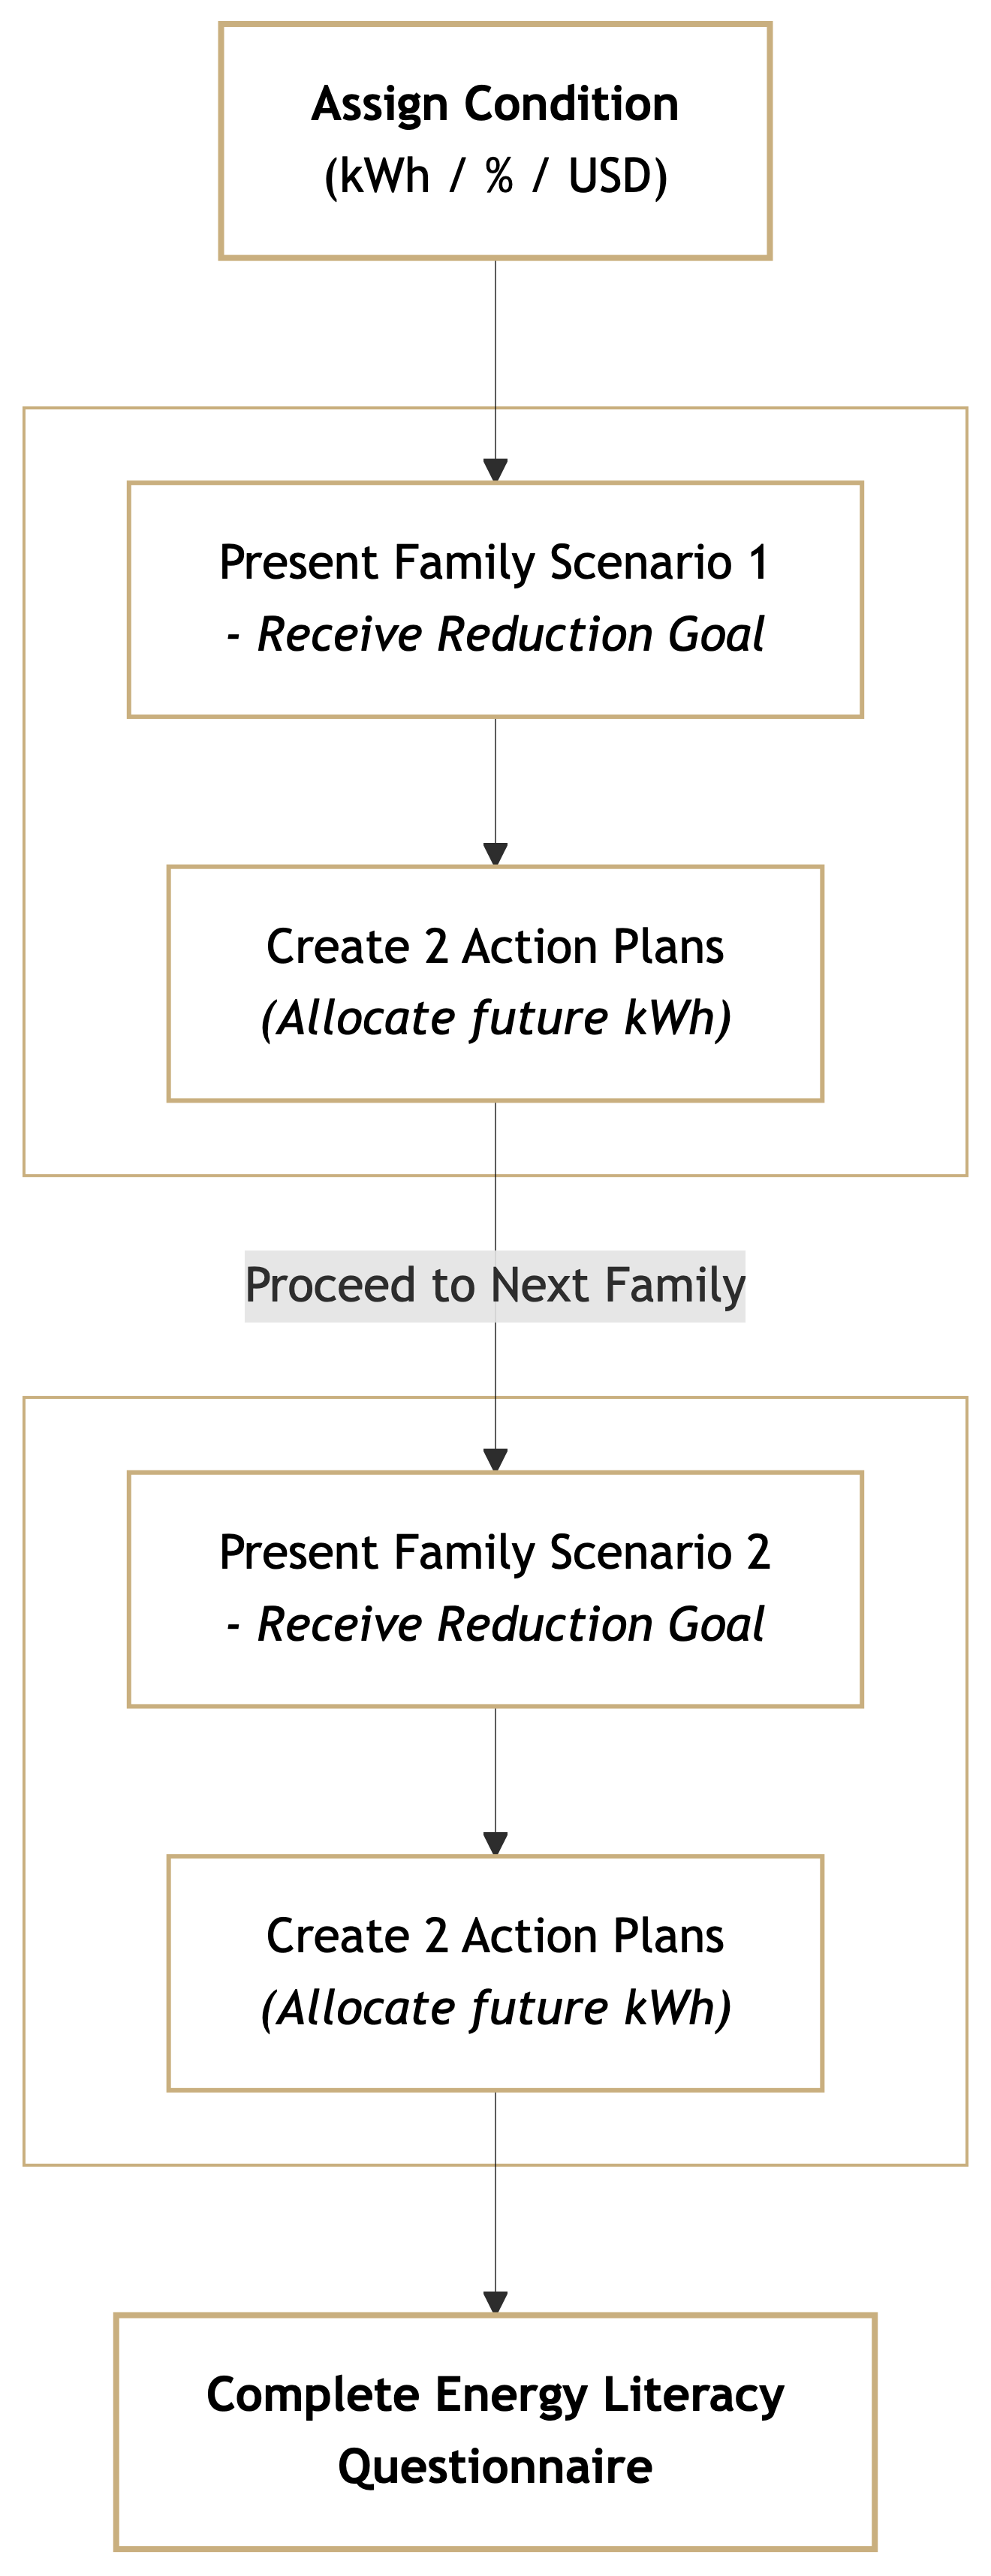
\includegraphics[width=\linewidth, height=9.5in,keepaspectratio]{assets/images/mermaid_proc.png}
    }
  \end{minipage}
  \hspace{0.5em}
  \begin{minipage}[t]{0.68\linewidth}
    \centering
    \subcaptionbox{Example of planning task interface \label{fig-task}}[0.95\linewidth]{%
      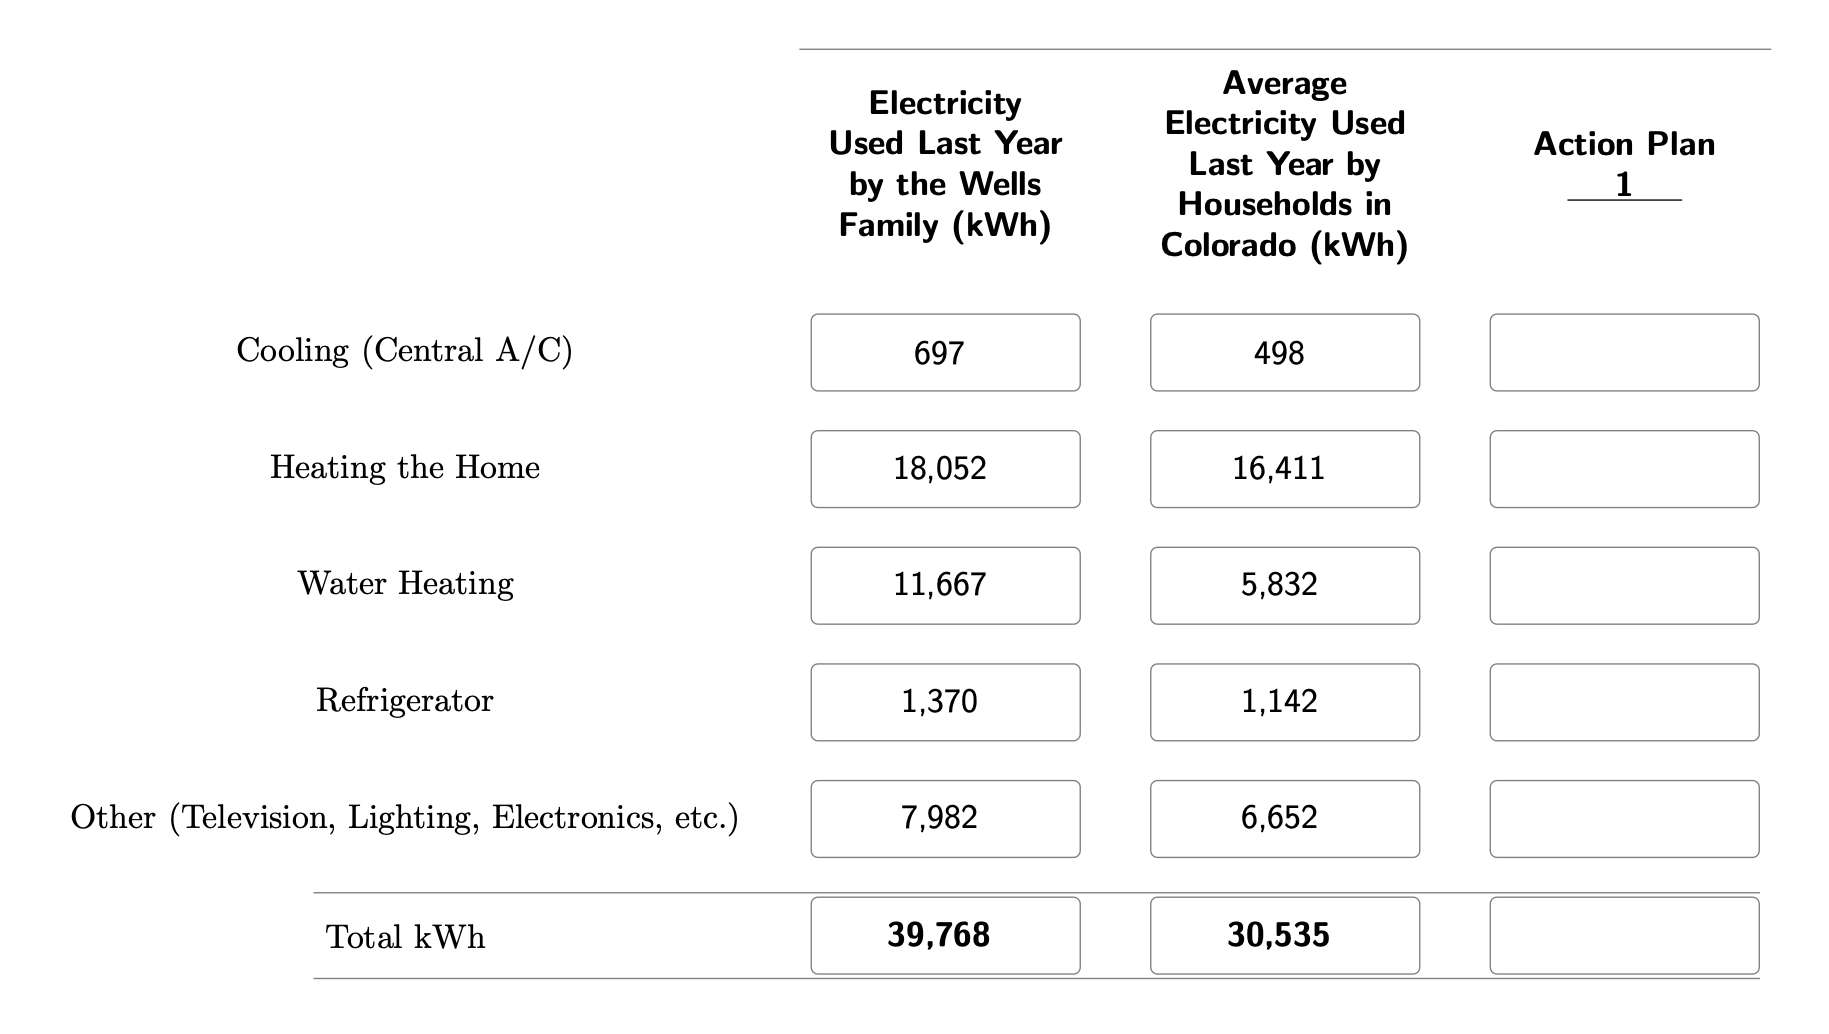
\includegraphics[width=\linewidth,height=9.5in, keepaspectratio]{assets/images/tab.png}
    }
  \end{minipage}
}

\end{figure}

\columnbreak

\subsection{Results}\label{results}

\begin{itemize}
\tightlist
\item
  \textbf{Key Measures:}

  \begin{itemize}
  \tightlist
  \item
    \textbf{Planning Accuracy:} Deviation between intended reduction
    goal and proposed plan (ordinal bins: exact, minor, large error).
  \item
    \textbf{Energy Literacy:} 8-item knowledge scale score (DeWaters \&
    Powers, 2011).
  \end{itemize}
\item
  \textbf{Analysis:} Bayesian mixed-effects regression:
  \(\text{Accuracy Level} \; \text{\textasciitilde} \; \text{Reference Class} + \text{Calculator} + (1|\text{id}) + (1|\text{Family Scenario})\)
\item
  \textbf{Effect of reference class (H1 Supported):} Smallest planning
  errors when reduction goal was presented in absolute units (kWh)
  compared to percentages (\%) or dollars (USD) across both experiments.
\item
  \textbf{Energy Literacy (H2 Supported):} Higher energy literacy scores
  associated with more accurate planning (lower error) in both
  experiments.
\end{itemize}

\subsubsection{Figure 2: Reference Class Effect on Planning Error (Exp
1)}\label{figure-2-reference-class-effect-on-planning-error-exp-1}

\begin{figure}[H]

{\centering 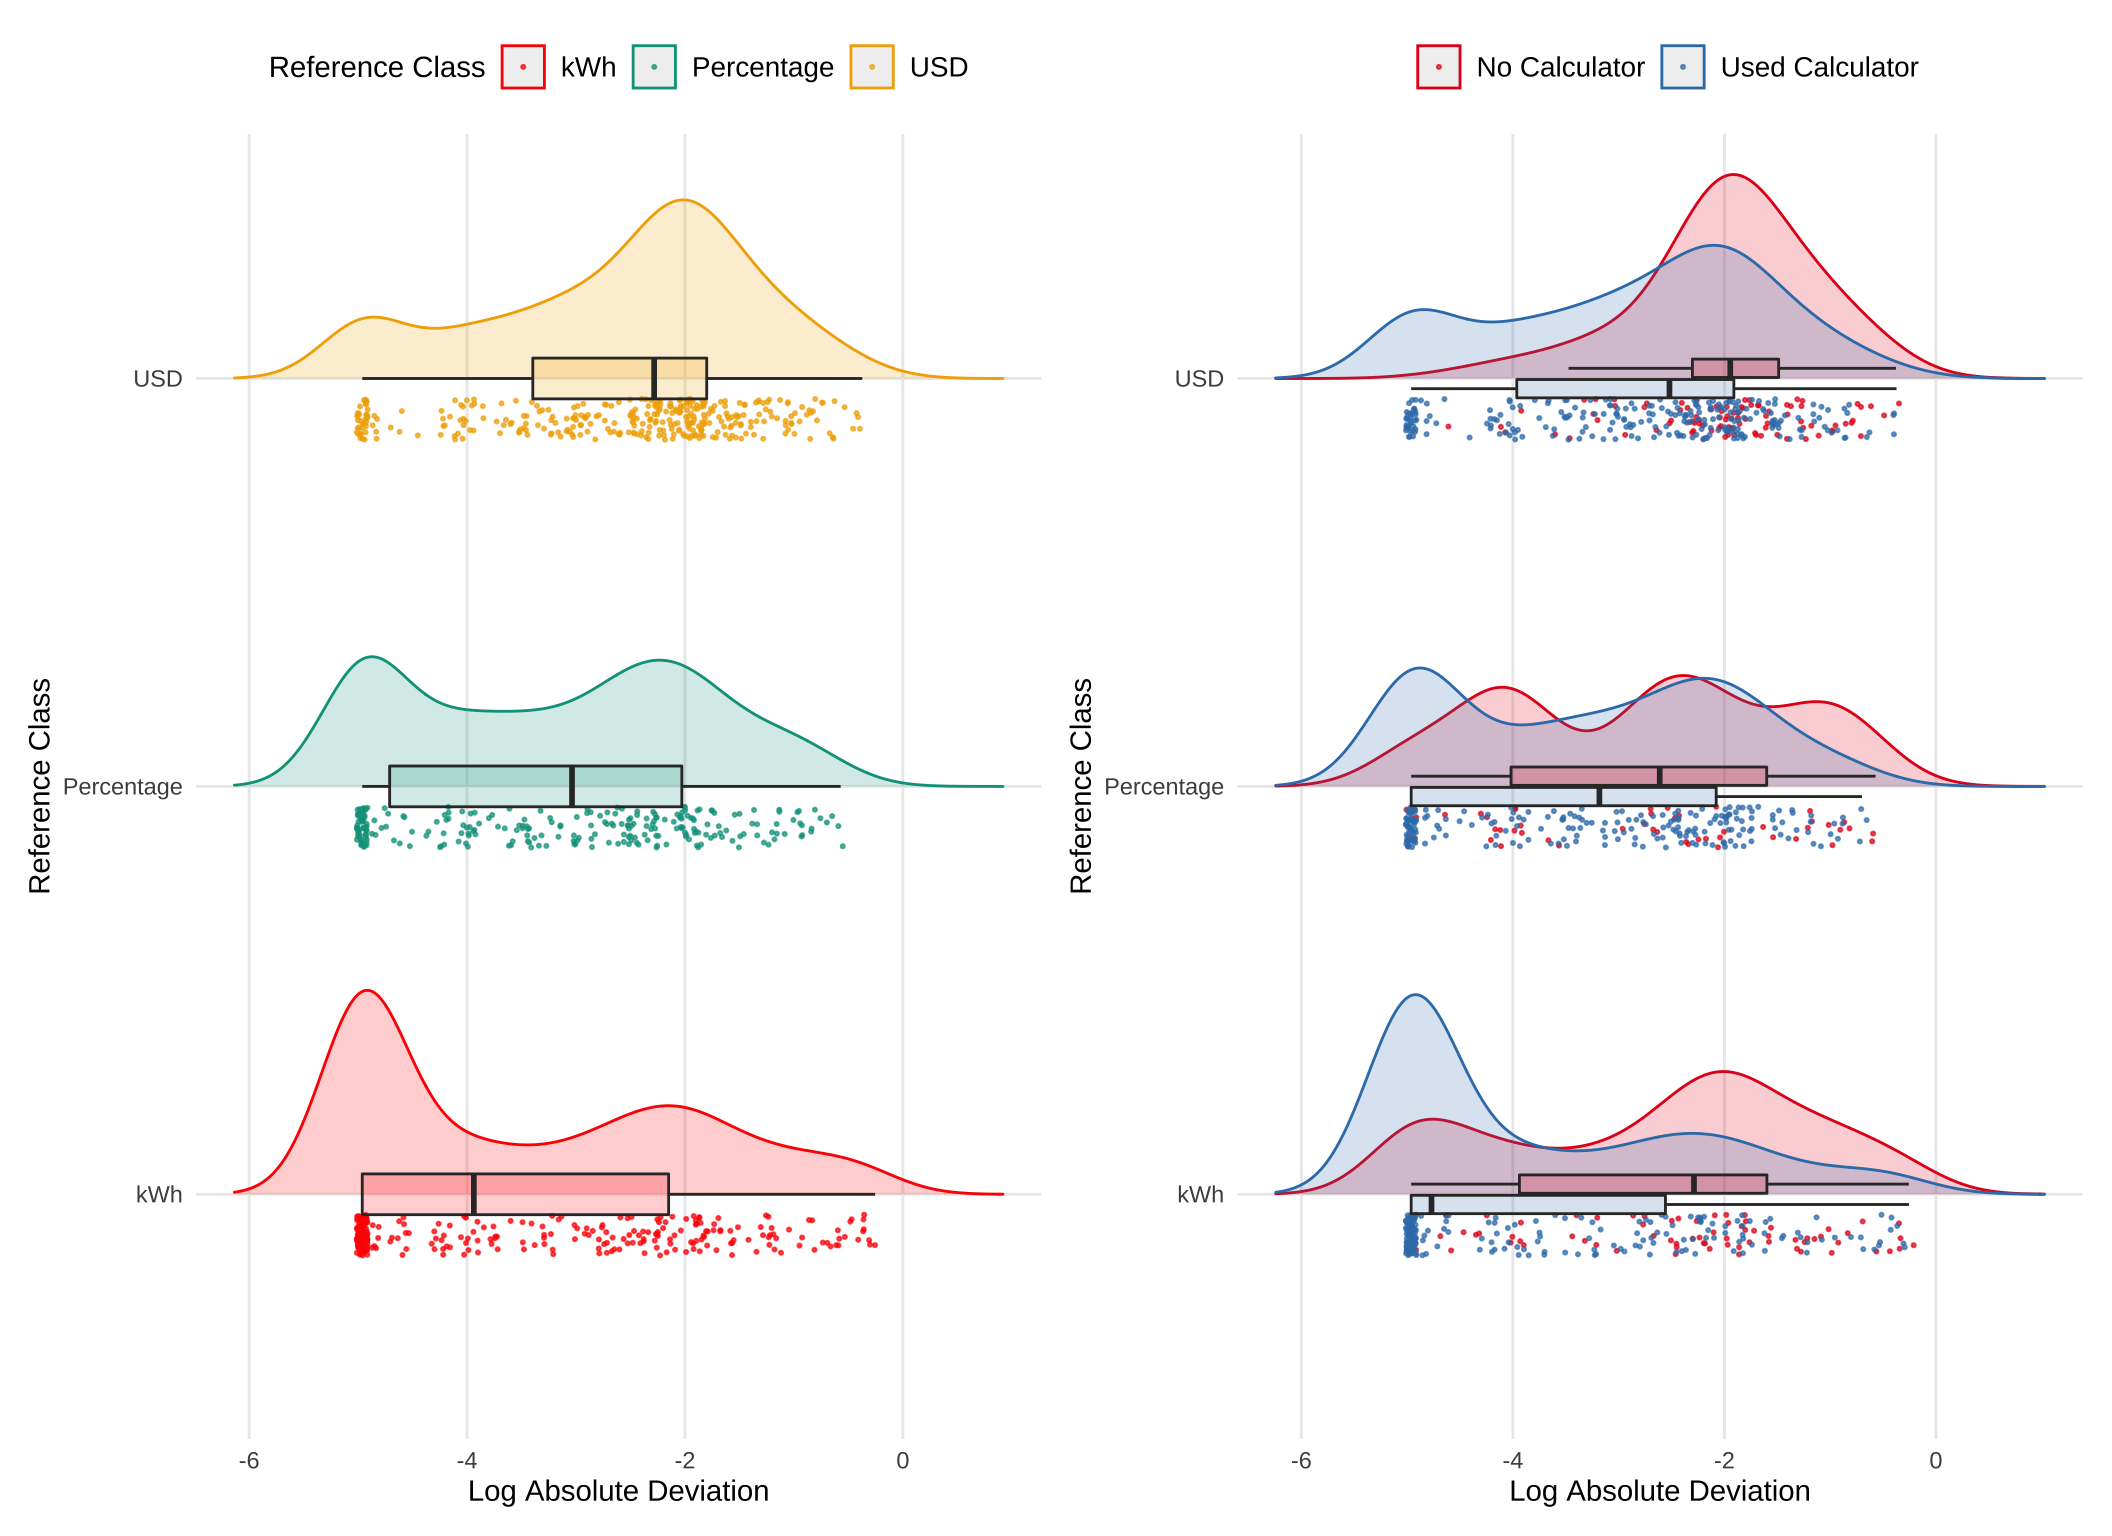
\includegraphics[width=0.85\linewidth,height=\textheight,keepaspectratio]{assets/images/fig-s1-log-dist-1.png}

}

\caption{Distribution of log absolute error by goal format condition
(Exp 1). Lower values indicate higher accuracy.}

\end{figure}%

\subsubsection{Figure 3 - Bayesian Regression Results (Exp
1)}\label{figure-3---bayesian-regression-results-exp-1}

\begin{figure}[H]
\centering

\makebox[\linewidth]{%
  \begin{minipage}[t]{0.44\linewidth}
    \centering
    \subcaptionbox{PPC for ordinal model. Blue bars are observed frequencies per accuracy level, dots show model predictions.\label{fig-s1-ppd}}[0.93\linewidth]{%
    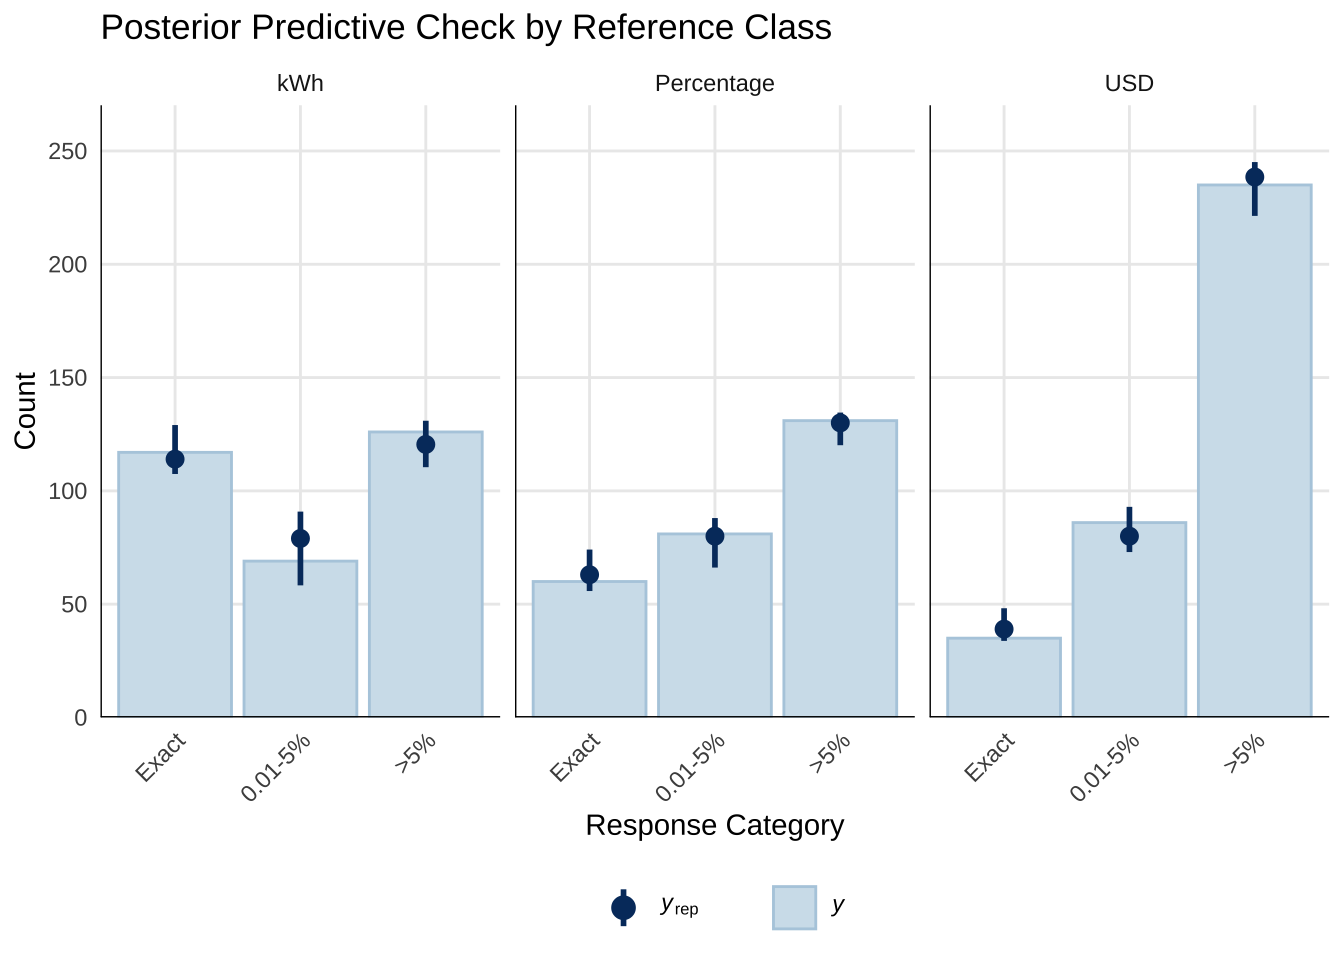
\includegraphics[height=4.4in, keepaspectratio]{assets/images/fig-s1-ppd-1.png}
    }
  \end{minipage}
  \hspace{0.01em}
  \begin{minipage}[t]{0.44\linewidth}
  \centering
    \subcaptionbox{Relationship between energy literacy score and log absolute error of reduction plans \label{fig-s1-els}}[0.93\linewidth]{%
    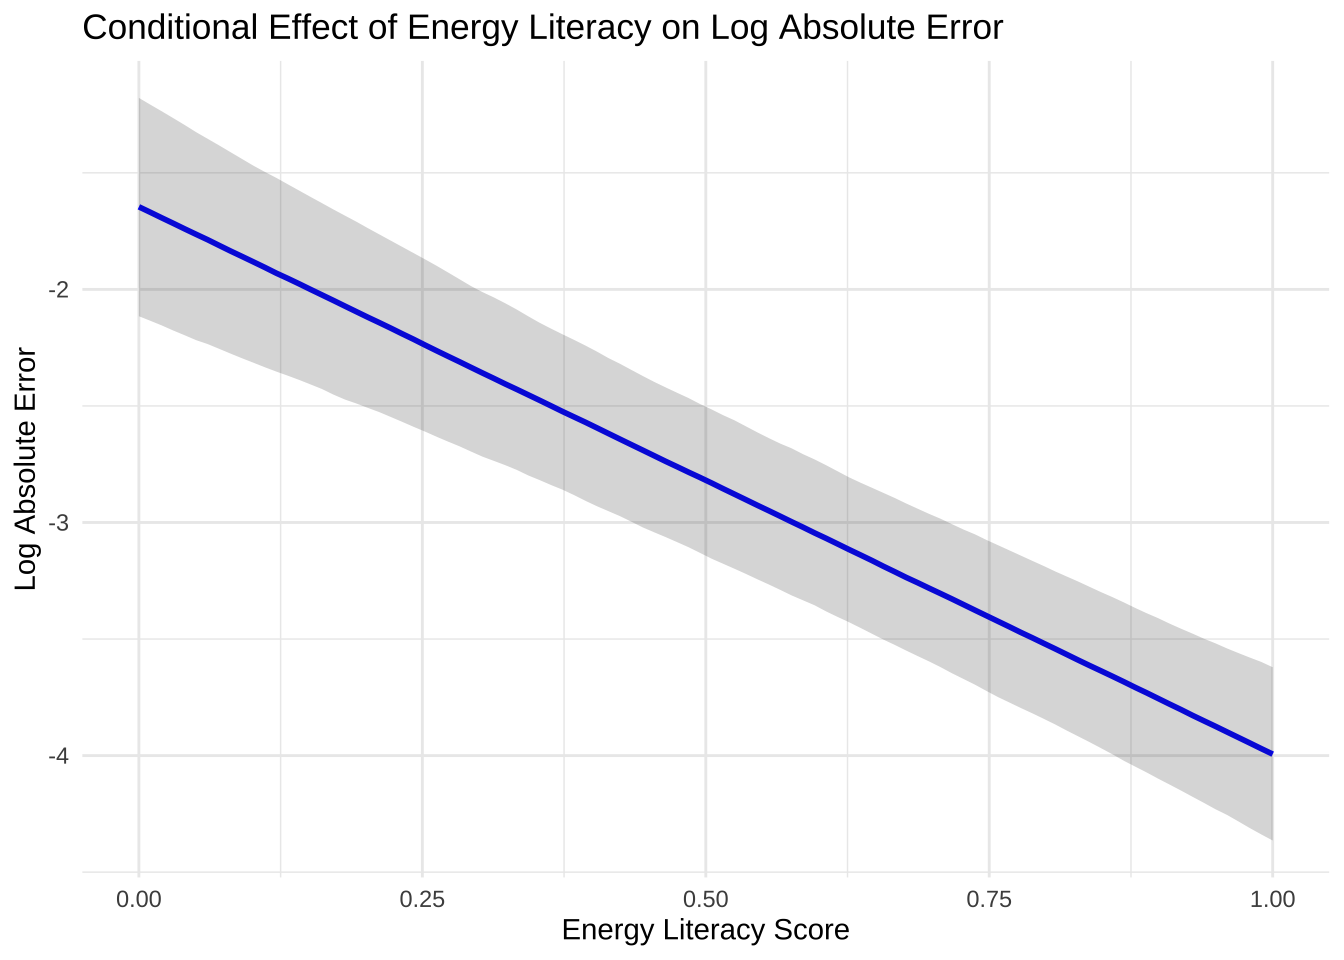
\includegraphics[height=4.4in, keepaspectratio]{assets/images/fig-s1-els-1.png}
    }
  \end{minipage}
}

\end{figure}

\columnbreak

\subsubsection{Figure 4: Reference Class Effect on Planning Error (Exp
2)}\label{figure-4-reference-class-effect-on-planning-error-exp-2}

\begin{figure}[H]

{\centering 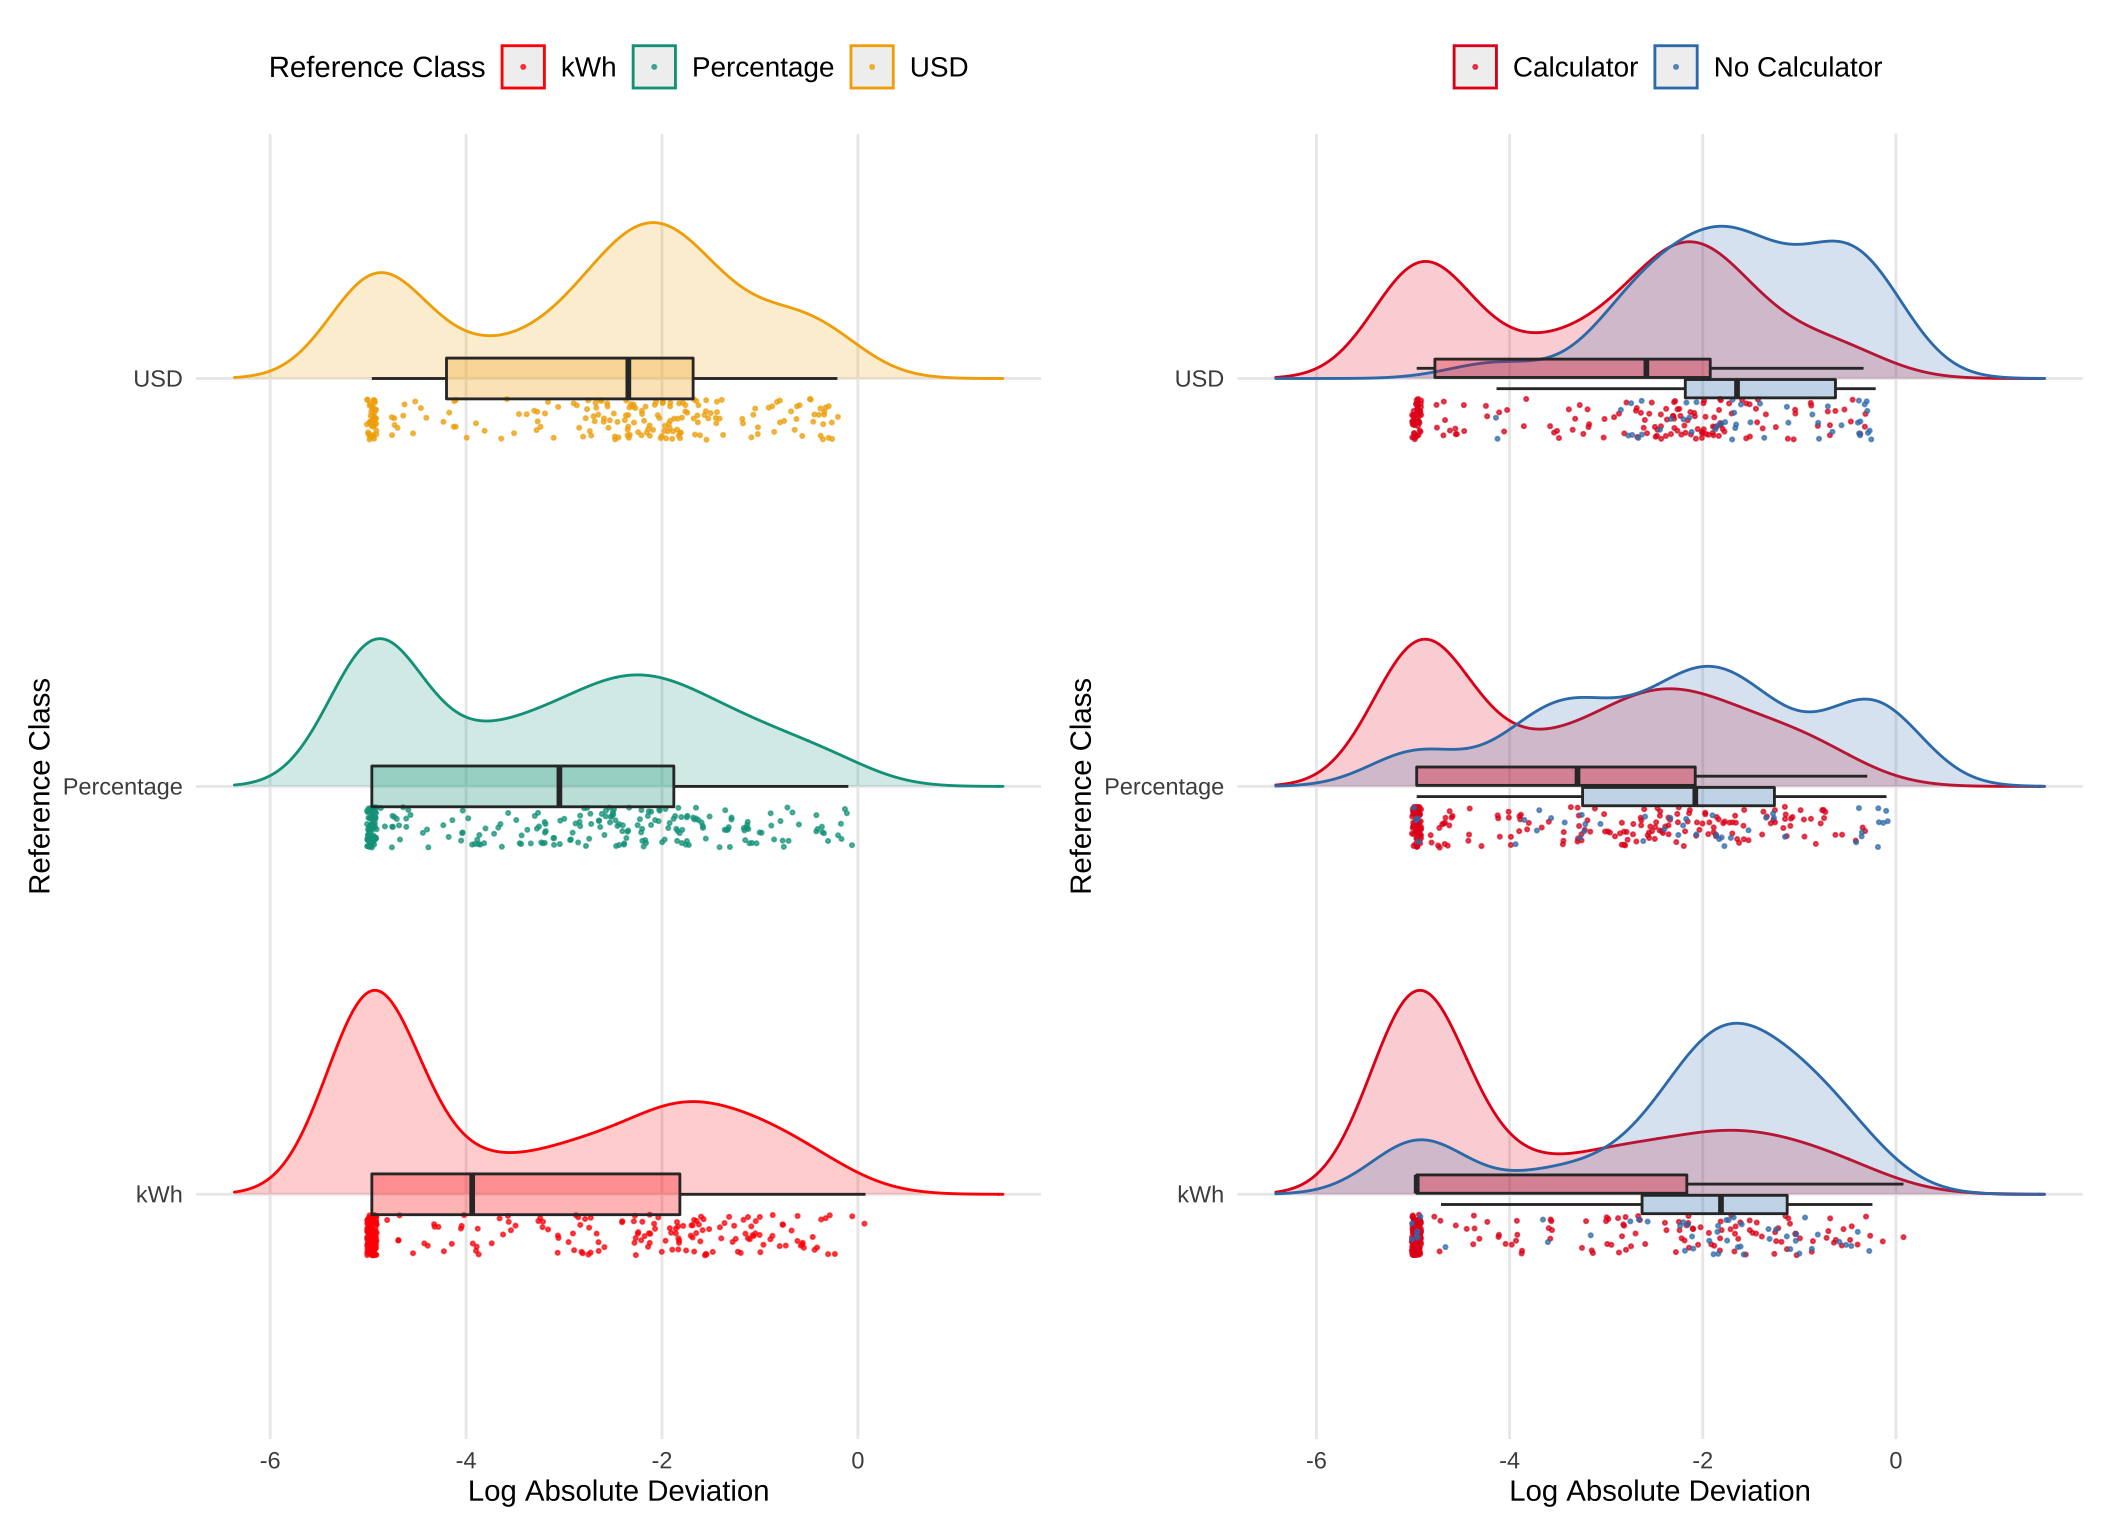
\includegraphics[width=0.85\linewidth,height=\textheight,keepaspectratio]{assets/images/fig-s2-log-dist-1.png}

}

\caption{Distribution of log absolute error by goal format condition
(Exp 2). Lower values indicate higher accuracy.}

\end{figure}%

\subsubsection{Figure 5 - Bayesian Regression Results (Exp
2)}\label{figure-5---bayesian-regression-results-exp-2}

\begin{figure}[H]
\centering

\makebox[\linewidth]{%
  \begin{minipage}[t]{0.44\linewidth}
    \centering
    \subcaptionbox{PPC for ordinal model. Blue bars are observed frequencies per accuracy level, dots show model predictions.\label{fig-s2-ppd}}[0.90\linewidth]{%
    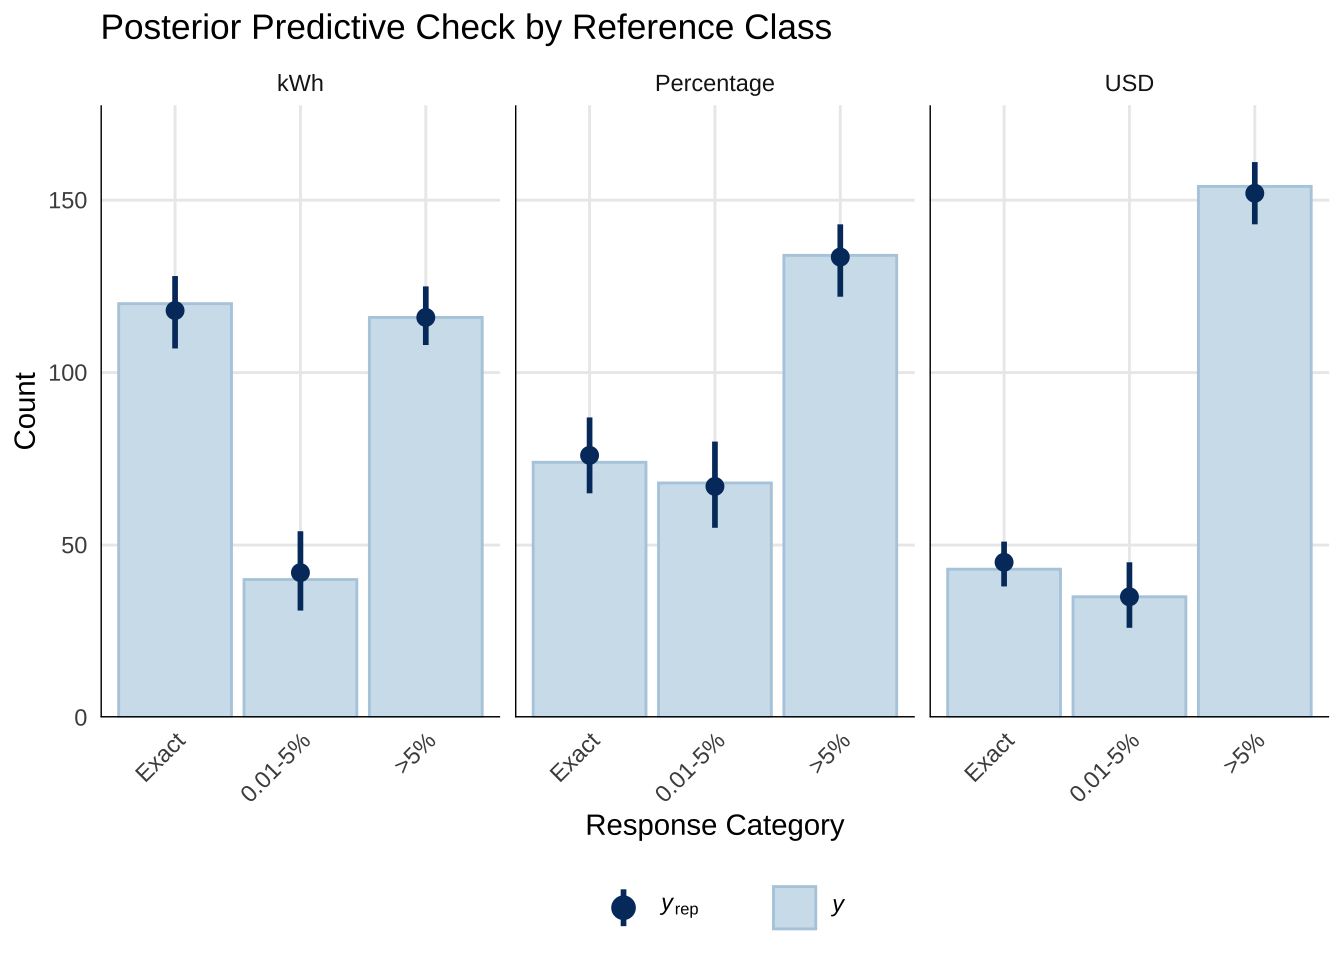
\includegraphics[height=4.4in, keepaspectratio]{assets/images/fig-s2-ppd-1.png}
    }
  \end{minipage}
  \hspace{0.01em}
  \begin{minipage}[t]{0.44\linewidth}
  \centering
    \subcaptionbox{Relationship between energy literacy score and log absolute error of reduction plans. \label{fig-s2-els}}[0.90\linewidth]{%
    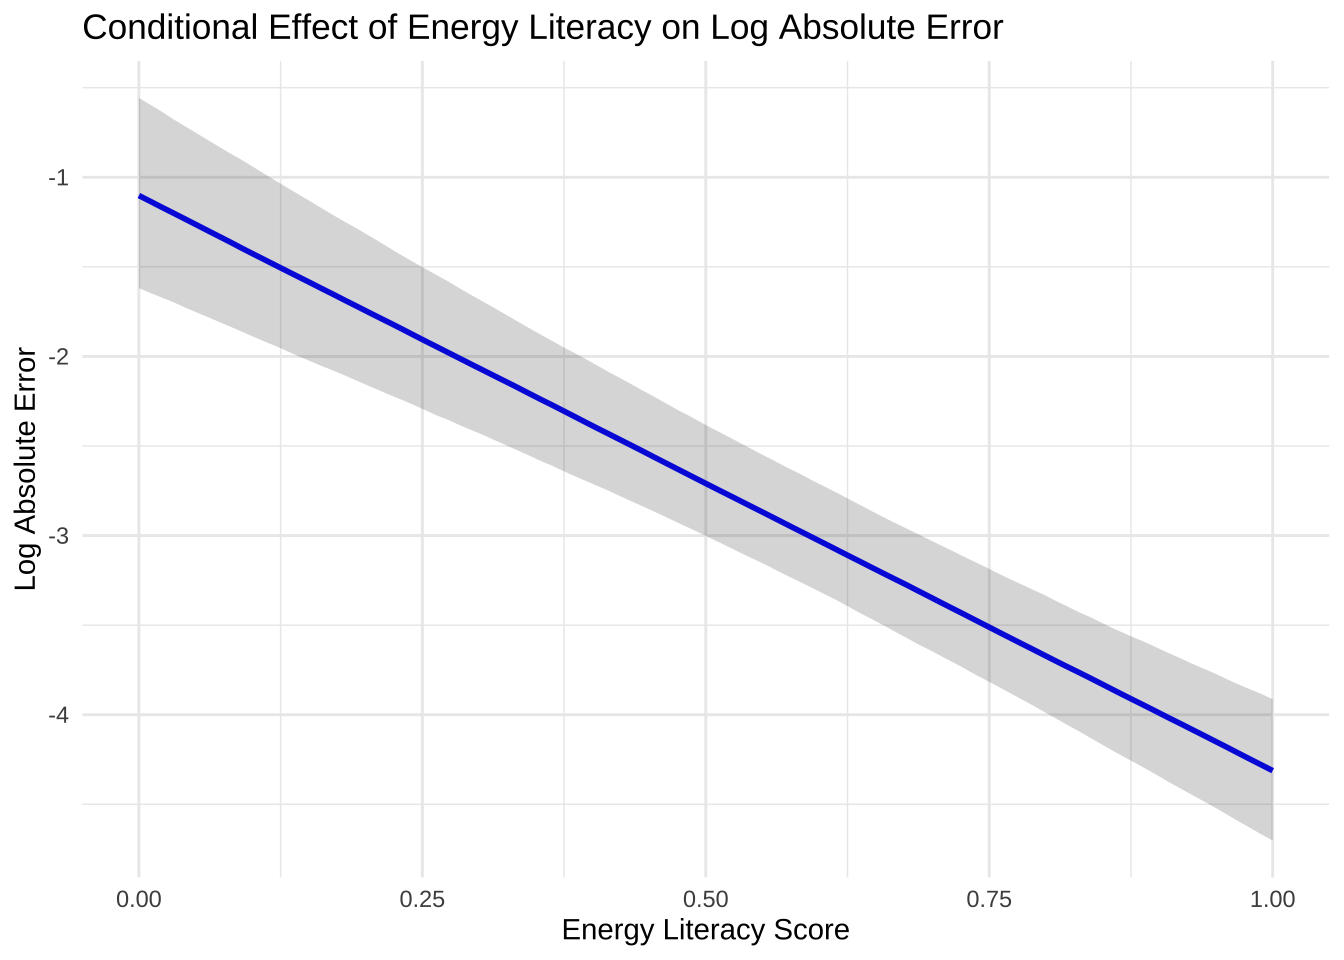
\includegraphics[height=4.4in, keepaspectratio]{assets/images/fig-s2-els-1.png}
    }
  \end{minipage}
}

\end{figure}

\subsection{Discussion}\label{discussion}

\begin{itemize}
\tightlist
\item
  \textbf{Key Finding:} Reference class significantly impacts planning
  accuracy. \textbf{Presenting goals in absolute kWh is superior} to
  relative (\%) or monetary (USD) formats, likely by simplifying
  calculations and reducing cognitive load.
\item
  \textbf{Energy Literacy Matters:} Higher domain knowledge consistently
  predicted better planning accuracy, emphasizing the role of energy
  education.
\item
  \textbf{Limitations:} Lab simulation, short duration, self-reported
  calculator use.
\end{itemize}

\subsection{References}\label{references}

\phantomsection\label{refs}
\begin{CSLReferences}{1}{0}
\bibitem[\citeproctext]{ref-bednarRecognitionResponseEnergy2020}
Bednar, D. J., \& Reames, T. G. (2020). Recognition of and response to
energy poverty in the {United States}. \emph{Nature Energy},
\emph{5}(6), 432--439. \url{https://doi.org/10.1038/s41560-020-0582-0}

\bibitem[\citeproctext]{ref-canfieldPerceptionsElectricityuseCommunications2017}
Canfield, C., Bruine De Bruin, W., \& Wong-Parodi, G. (2017).
Perceptions of electricity-use communications: Effects of information,
format, and individual differences. \emph{Journal of Risk Research},
\emph{20}(9), 1132--1153.
\url{https://doi.org/10.1080/13669877.2015.1121909}

\bibitem[\citeproctext]{ref-dewatersEnergyLiteracySecondary2011}
DeWaters, J. E., \& Powers, S. E. (2011). Energy literacy of secondary
students in {New York State} ({USA}): {A} measure of knowledge, affect,
and behavior. \emph{Energy Policy}, \emph{39}(3), 1699--1710.
\url{https://doi.org/10.1016/j.enpol.2010.12.049}

\bibitem[\citeproctext]{ref-fischerFeedbackHouseholdElectricity2008}
Fischer, C. (2008). Feedback on household electricity consumption: A
tool for saving energy? \emph{Energy Efficiency}, \emph{1}(1), 79--104.
\url{https://doi.org/10.1007/s12053-008-9009-7}

\bibitem[\citeproctext]{ref-gigerenzerSimpleToolsUnderstanding2003}
Gigerenzer, G., \& Edwards, A. (2003). Simple tools for understanding
risks: From innumeracy to insight. \emph{BMJ}, \emph{327}(7417),
741--744. \url{https://doi.org/10.1136/bmj.327.7417.741}

\bibitem[\citeproctext]{ref-memmottSociodemographicDisparitiesEnergy2021}
Memmott, T., Carley, S., Graff, M., \& Konisky, D. M. (2021).
Sociodemographic disparities in energy insecurity among low-income
households before and during the {COVID-19} pandemic. \emph{Nature
Energy}, \emph{6}(2), 186--193.
\url{https://doi.org/10.1038/s41560-020-00763-9}

\bibitem[\citeproctext]{ref-reimerNumericCommunicationRisk2015}
Reimer, T., Jones, C., \& Skubisz, C. (2015). Numeric {Communication} of
{Risk}. In \emph{The {SAGE} handbook of risk communication} (pp.
167--179).

\end{CSLReferences}



% This part runs after the main document content

\end{multicols} % End the 3-column layout

% Draw a simple footer line with a slightly taller background
\AddToHook{shipout/background}{% Add to background hook for each page
  \begin{tikzpicture}[remember picture, overlay]
    % Extend footer area height slightly
    \fill[purduegold] (current page.south west) rectangle ([yshift=0.53in]current page.south east); 

    % Adjust Text position in the footer
    \node[anchor=south east, xshift=-0.75in, yshift=0.2in, % Shift down slightly
          text=darkgray, font=\small\sffamily] % Text color and font
          at (current page.south east) 
          {Communication and Cognition Lab | Purdue University}; 
          
    % Adjust email position in the footer
    \node[anchor=south west, xshift=0.75in, yshift=0.05in, % Shift down slightly
          text=darkgray, font=\small\sffamily] % Text color and font
          at (current page.south west) 
          {\textsuperscript{*}Corresponding author: \href{mailto:tegorman@purdue.edu}{tegorman@purdue.edu}};
  \end{tikzpicture}
}

% \end{multicols} % End the 3-column layout

% % Draw background color and text for footer area using TikZ overlay
% \AddToHook{shipout/background}{% Add to background hook for each page
%   \begin{tikzpicture}[remember picture, overlay]
%     % Fill footer area with Purdue Gold - adjust height (1in) as needed
%     \fill[purduegold] (current page.south west) rectangle ([yshift=0.8in]current page.south east); 

%     % Add Text to the footer - Adjust position and content
%     \node[anchor=south east, xshift=-0.75in, yshift=0.25in, % Position from bottom right
%           text=darkgray, font=\small\sffamily] % Text color and font
%           at (current page.south east) 
%           {Communication and Cognition Lab | Purdue University}; 
          
%     % Add email to the left side of the footer
%     \node[anchor=south west, xshift=0.75in, yshift=0.25in, % Position from bottom left
%           text=darkgray, font=\small\sffamily] % Text color and font
%           at (current page.south west) 
%           {\textsuperscript{*}Corresponding author: \href{mailto:tegorman@purdue.edu}{tegorman@purdue.edu}};
          
%     % Optional: Add a logo - Uncomment and adjust path/size
%     % \node[anchor=south west, xshift=0.75in, yshift=0.15in] 
%     %       at (current page.south west) {
%     %   \includegraphics[height=0.5in]{path/to/purdue_logo.png} % Adjust height/path
%     % };
%   \end{tikzpicture}
% }
\end{document}
